%----------------------------------------------------------------------------------------
%  Verbalizable Causal Channels Are Model- and Task-Dependent in Open Language Models
%
%  Fresh paper start (2026-07-30). NOT derived from the run handouts — those are
%  frozen run-era artifacts. Prose here is written new against the registered
%  evidence. Every quantitative claim carries its evidence id in a trailing
%  \eid{...} bracket (the registry is interpretability/jspace_phase3/reports/
%  evidence_events.jsonl); numbers were independently re-derived from the
%  item-level parquets by interpretability/jspace_runs/analysis/run_analysis.py.
%
%  Template: adapted from kburtram_report.tex (CSEP 590A Sp26 report).
%----------------------------------------------------------------------------------------

\documentclass[twoside,twocolumn]{article}

\usepackage{graphicx}
\usepackage[sc]{mathpazo}
\usepackage[T1]{fontenc}
\linespread{1.05}
\usepackage{microtype}

\widowpenalty=10000
\clubpenalty=10000
\raggedbottom
\setlength{\emergencystretch}{3em}
\usepackage{amsmath,amssymb}
\usepackage[english]{babel}

\usepackage[hmarginratio=1:1,top=32mm,columnsep=20pt]{geometry}
\usepackage[hang, small,labelfont=bf,up,textfont=it,up]{caption}
\usepackage{booktabs}
\usepackage{float}
\usepackage{url}
\usepackage{placeins}
\usepackage{dblfloatfix}
\usepackage{lettrine}
\usepackage{enumerate}
\usepackage{enumitem}
\setlist[itemize]{noitemsep}
\usepackage{xcolor}

\usepackage{abstract}
\renewcommand{\abstractnamefont}{\normalfont\bfseries}
\renewcommand{\abstracttextfont}{\normalfont\small\itshape}

\usepackage{titlesec}
\renewcommand\thesection{\Roman{section}}
\renewcommand\thesubsection{\roman{subsection}}
\titleformat{\section}[block]{\large\scshape\centering}{\thesection.}{1em}{}
\titleformat{\subsection}[block]{\large}{\thesubsection.}{1em}{}

\usepackage{fancyhdr}
\pagestyle{fancy}
\fancyhead{}
\fancyfoot{}
\fancyfoot[RO,LE]{\thepage}

\usepackage{titling}
\usepackage{hyperref}
\hypersetup{hidelinks}

% --- paper-local macros ---------------------------------------------------
\newcommand{\eid}[1]{{\footnotesize\texttt{[#1]}}}          % evidence id
\newcommand{\tier}[1]{{\footnotesize\textsc{(#1)}}}          % tier watermark
\newcommand{\todo}[1]{{\color{red!70!black}\textbf{[TODO: #1]}}}

\makeatletter
\renewcommand{\p@subsection}{\thesection.}
\setlength{\@fpsep}{\baselineskip}
\makeatother

\setlength{\droptitle}{-6\baselineskip}

\pretitle{\begin{center}\LARGE\bfseries}
\posttitle{\par\end{center}\vskip 0.2em}
\title{Verbalizable Causal Channels Are Model- and Task-Dependent\\in Open Language Models}
\preauthor{\begin{center}\normalsize}
\postauthor{\end{center}}
\author{\textsc{Karl Burtram} \,\textperiodcentered\, University of Washington \,\textperiodcentered\, \href{mailto:kburtram@uw.edu}{kburtram@uw.edu}}
\date{}
\setlength{\absleftindent}{0pt}
\setlength{\absrightindent}{0pt}
\renewcommand{\maketitlehookd}{%
\vspace*{-2em}%
\begin{abstract}
\noindent
A 2026 interpretability result proposes that the verbalizable subspace
read out by a fitted Jacobian lens forms a \emph{global workspace} in
language models: sparse, broadcast, and causally privileged, such that
deleting its content selectively destroys multi-step behavior while
sparing direct recall.  This paper reports a three-phase, preregistered
replication program on open-weights models (OLMo~3.1~32B Think and
Instruct; Qwen~3.6~27B) whose central technical finding is about the
\emph{instrument}: the paper's output-protection contract protects
output \emph{labels}, not output \emph{geometry}, and 28--42\% of the
activation energy removed by the ``protected'' ablation lies inside the
protected output span.  Under a span-safe arm that removes this leak by
construction, a J-specific heavy tail of per-item damage survives at
confirmatory tier on Qwen (tail-rate excess $+0.096$ over an exactly
rank-and-energy-matched control, $p\approx10^{-5}$; independent
replication $+0.102$) at roughly one third of its label-protected size.
A preregistered bridge-protection test confirms mediation on Qwen:
protecting the true intermediate (``bridge'') entity's directions
rescues composed-item damage by $+0.43$ nats relative to a matched
counterfactual bridge, and substituting the counterfactual bridge's
content at matched dose is catastrophically worse than deletion
($-4.05$ nats) --- the model demonstrably reads what sits in the
channel.  OLMo shows none of this: its damage is organized by answer
accessibility rather than task shape, and its rescue contrast is mildly
negative.  The workspace-word test fails on both clusters --- the
composed-vs-direct contrast does not appear on in-context task banks
--- so the supportable noun is \emph{knowledge-access channel}, not
workspace.  All primary quantities reproduce clean-room from frozen
raw data to $\le 5\times10^{-4}$, including one full GPU cell
bit-exactly.
\end{abstract}
}

\begin{document}

\maketitle
\thispagestyle{empty}

%----------------------------------------------------------------------------------------
\section{The Problem}\label{sec:problem}

\lettrine[nindent=0em,lines=2]{T}{he} claim under test comes from the
July-2026 paper \emph{``Verbalizable Representations Form a Global
Workspace in Language Models''}~\cite{Anthropic:Workspace}: a small,
verbalizable subspace of the residual stream --- read out by a fitted
Jacobian lens~\cite{Anthropic:JLens} --- is \emph{causally privileged},
such that deleting its content selectively destroys composed (multi-hop)
behavior while sparing direct recall.  The claim matters because it is
the strongest mechanistic-interpretability result to date connecting a
\emph{readable} representation to a \emph{causally load-bearing} one,
and because ``workspace'' imports a functional architecture --- a shared
bus between specialist processes --- that circuits-level results do not
usually claim.

\todo{1--2 paragraphs situating the replication program: Phase 1
exploratory lab (superseded by errata), Phase 2 preregistered
confirmatory campaign on the audited assay, Phase 3 mechanism +
generalization.  Cite the governing preregistrations.}

Separating ``the model lost the fact'' from ``the model lost the
ability to say anything'' from ``the model was injured proportionally
to how much of anything was removed'' is the entire technical problem;
\S\ref{sec:repair} shows that each confusion occurred in practice and
was caught by an instrument audit.

%----------------------------------------------------------------------------------------
\section{Assay Repair}\label{sec:repair}

\todo{Port the assay-repair story: each repair exists because an
instrument fault produced, or would have produced, a false claim.}

\begin{itemize}
  \item \textbf{Output protection done properly.}  Per-position
  exclusion of the clean top-$k$ token rows from J-selection; the open
  question it leaves --- label exclusion bounds \emph{selection}, not
  \emph{geometry} --- becomes \S\ref{sec:leak}.
  \item \textbf{The exact instantaneous rank-and-energy matched
  control.}  Per (item, layer, position), a random subspace matching
  the J arm's achieved effective rank and removed energy exactly,
  orthogonal to the protected rows
  \eid{mc-dev-validation-olmo31-think-v2}.  At matched dose, direction
  content is the only difference between arms.
  \item \textbf{One unit system.}  Two tokenizer-convention faults
  (BOS units; concatenation) caught by the preregistered stop rule
  before any confirmatory outcome was viewed
  \eid{AMENDMENT\_1\_BOS\_UNITS}.
  \item \textbf{Audited families.}  Hand-audited item families replace
  a string-split accident; every clustered statistic runs on the
  audited map.
  \item \textbf{Positive controls.}  G4 swap controls certify each
  lens causally (flip rate $0.76$--$0.78$ vs $0.18$--$0.24$ random)
  \eid{r5-swap-positive-control-*-v2}.
\end{itemize}

%----------------------------------------------------------------------------------------
\section{The Phase 2 Confirmatory Matrix}\label{sec:phase2}

\todo{Frozen Phase 2 results, stated with the thin-two-hop limitation
first.  Primary outcomes: HP1 composed-minus-direct contrast $-0.504$
$[-0.720, -0.295]$, $p_{\mathrm{holm}}=5\times10^{-4}$; HP3 J-specific
tail excess $+0.279$ $[+0.205, +0.361]$ (Qwen)
\eid{n6-confirmatory-analysis-v2}.  Held-out replication: HP3
replicates ($+0.297$); HP1 inconclusive on the 9-item two-hop leg.
Corrected capacity: Qwen at $5$--$6\%$ centered excess (lower edge of
the reported Claude band), the OLMo 3.1 pair flat at $\sim$$1.2\%$
\eid{r2-occupancy-*-v2}.}

%----------------------------------------------------------------------------------------
\section{Label Protection Is Not Span Protection}\label{sec:leak}

The opening question of Phase 3 --- does protecting output token
\emph{labels} from selection keep the removed span away from output
\emph{geometry}? --- has a sharp answer: no, on every model tested.
Under label protection the selected J span overlaps the protected span
(projector overlap $0.89$/$0.94$/$1.37$ for Think/Instruct/Qwen), a
large share of removed activation energy sits inside the protected span
($37\%$/$42\%$/$28\%$), and the never-selectable answer direction loses
$18$--$26\%$ of its norm \eid{p3-span-audit-cross-model-v1}
\tier{phase3-development}.  A span-safe arm zeroes the overlap exactly.

The behavioral consequence decomposes differently per model
(Fig.~\ref{fig:labelspan}): on the OLMo pair the label-protected and
span-safe arms damage substantially \emph{different} items (per-item
$r=0.20$/$0.29$) --- a reallocation --- while on Qwen $r=0.75$ and the
leakage-dose control is nil: Qwen's label-protected effect was mostly
content all along.

\begin{figure*}[tbp]
  \centering
  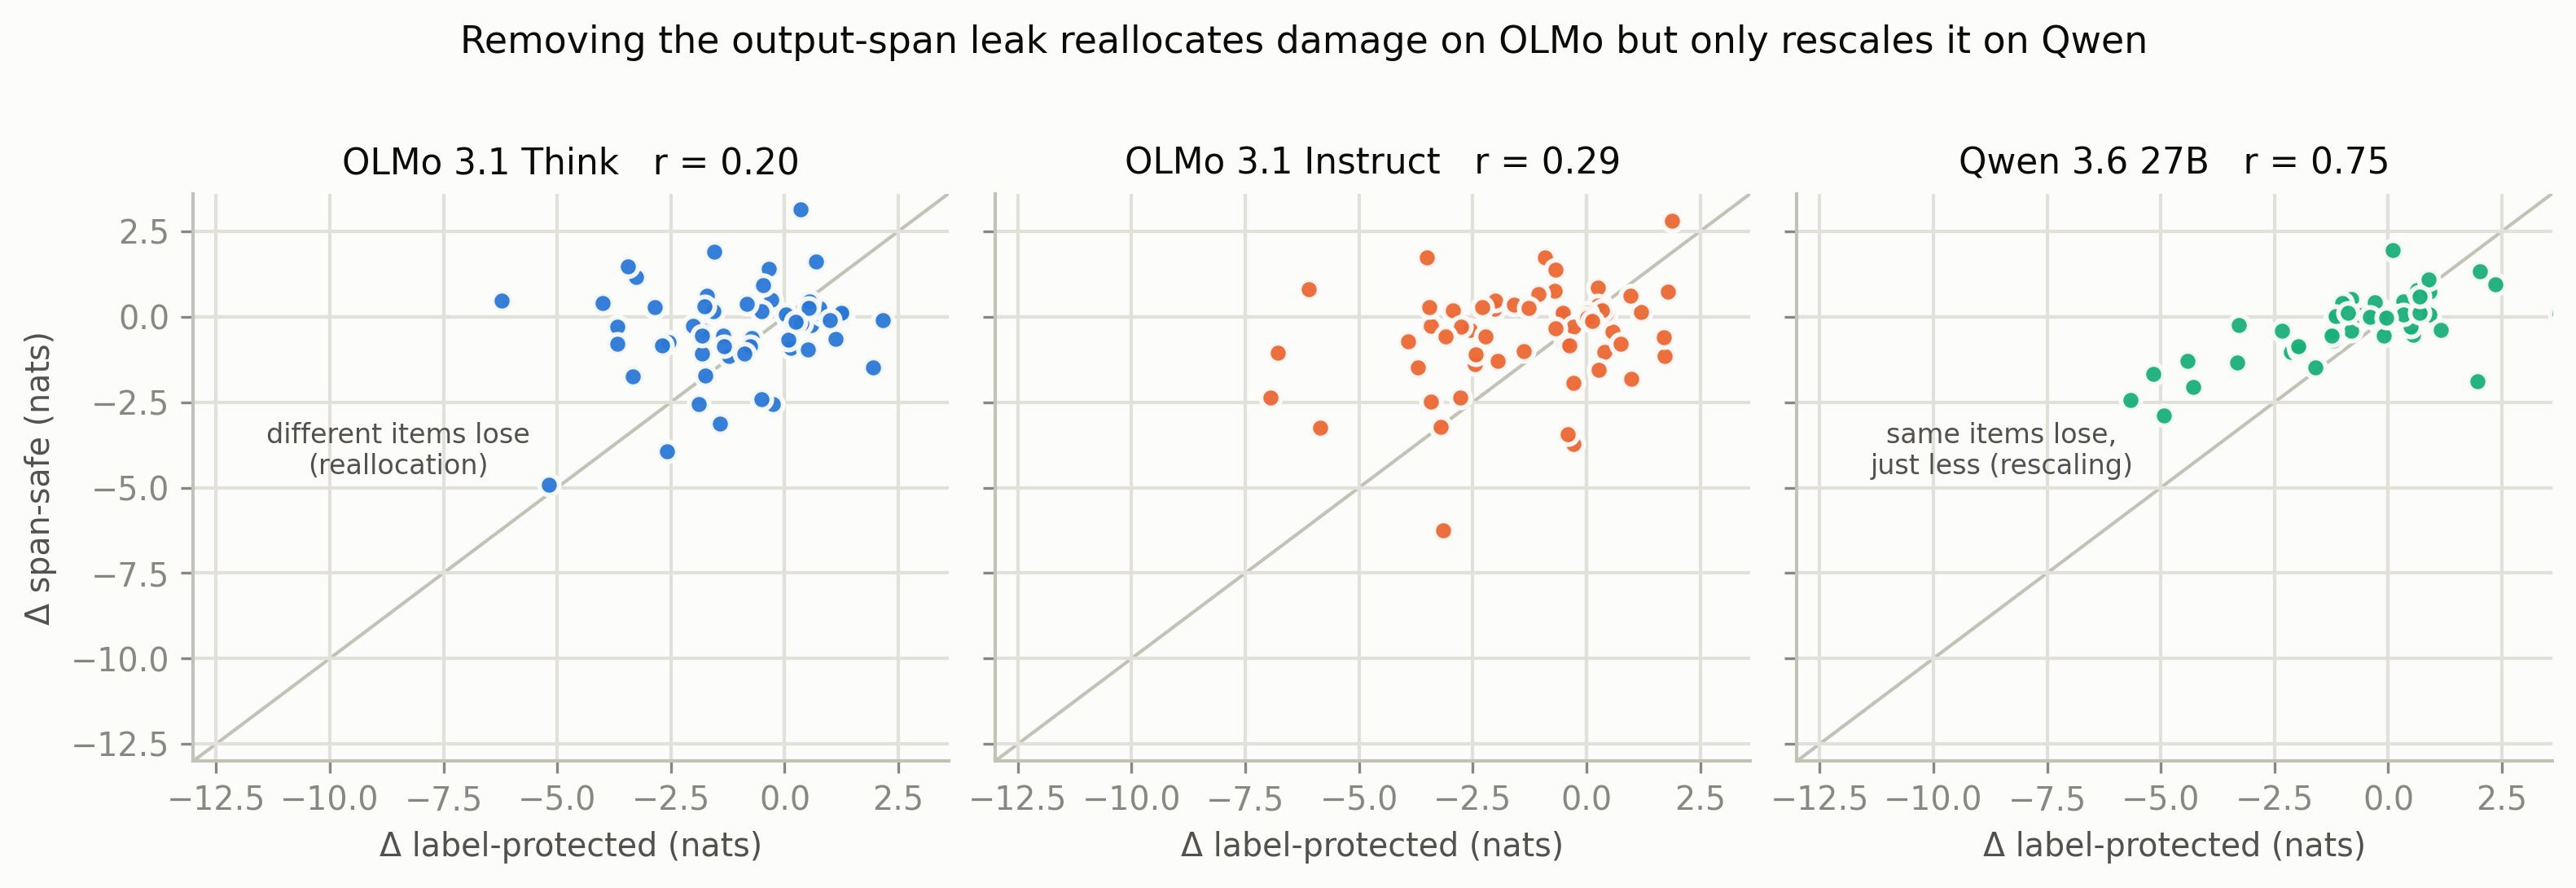
\includegraphics[width=\linewidth]{figures/figB_label_vs_spansafe.png}
  \caption{Per-item damage under the paper-faithful label-protected arm
  ($x$) vs the leak-free span-safe arm ($y$), on the 60 frozen Phase 2
  confirmatory items per model.  Removing the output-span leak
  \emph{reallocates} damage on OLMo ($r=0.20$/$0.29$) and merely
  \emph{rescales} it on Qwen ($r=0.75$)
  \eid{p3-span-audit-cross-model-v1} \tier{phase3-development}.}
  \label{fig:labelspan}
\end{figure*}

\subsection{The specificity claim survives the repair}\label{sec:p3p2}

The campaign's central specificity claim was re-established at
confirmatory tier with the leak removed by construction: on Qwen, the
span-safe J-specific tail-rate excess over the exact matched control is
$+0.096$ ($188$ items, $26$ families, $p\approx10^{-5}$)
\eid{p3-locked-analysis-v1} \tier{phase3-confirmatory}, and
independently replicates at $+0.102$ on disjoint held-out families
\eid{p3-replication-analysis-v1} \tier{phase3-replication} ---
about one third of the label-protected effect, quantitatively
consistent with the leakage/content decomposition
(Figs.~\ref{fig:ecdf},~\ref{fig:eras}).

\begin{figure*}[tbp]
  \centering
  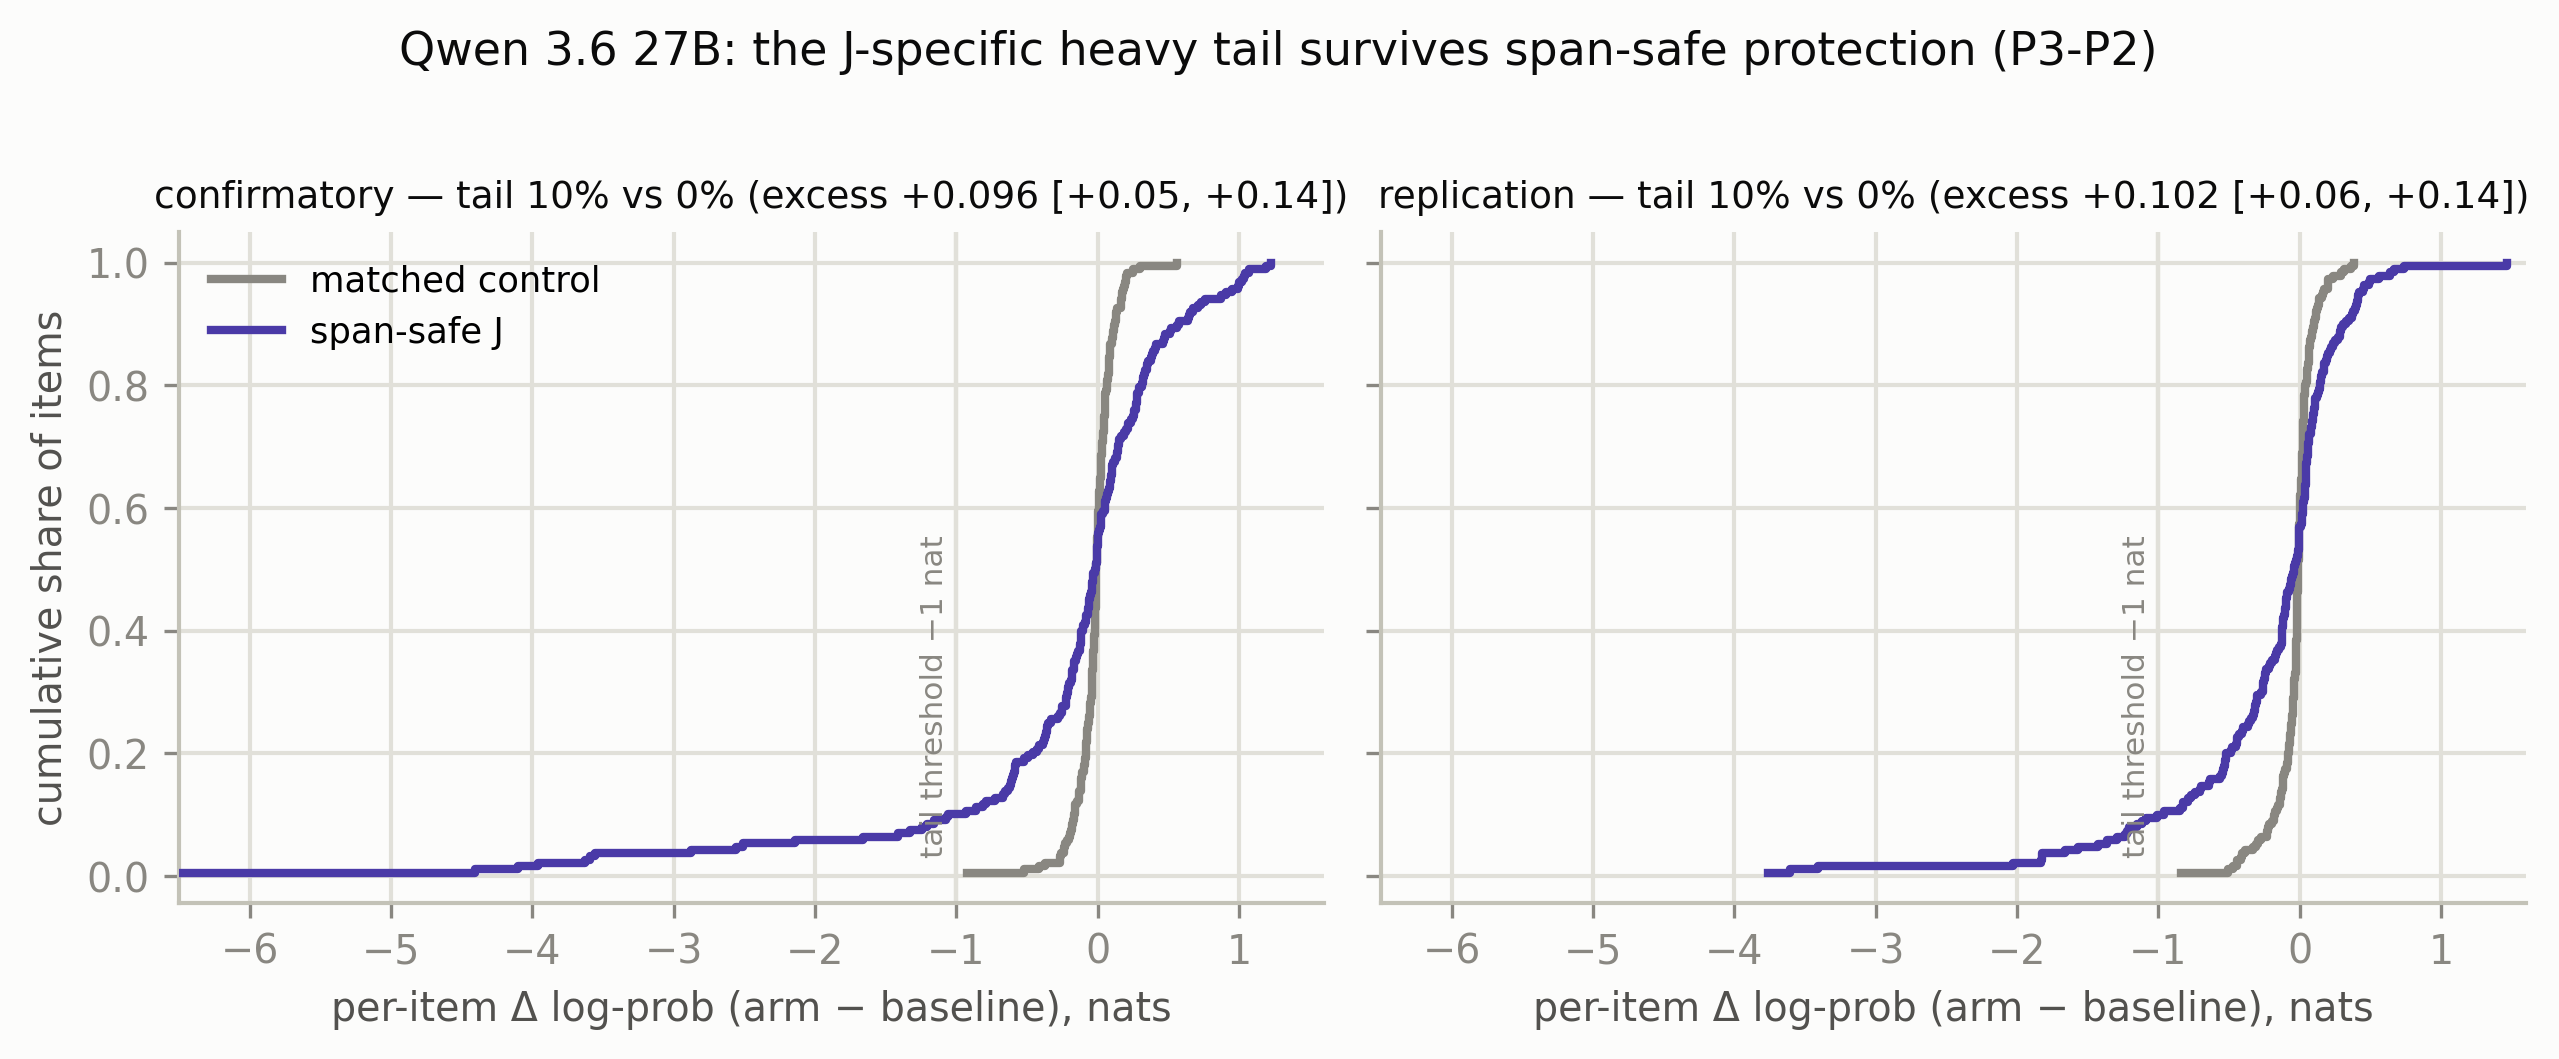
\includegraphics[width=\linewidth]{figures/figA_p3p2_ecdf.png}
  \caption{Per-item damage distributions on Qwen under span-safe J
  ablation vs the exact rank-and-energy matched control, confirmatory
  (left) and held-out replication (right).  The control produces no
  $-1$-nat tail; the J arm's tail survives full span protection
  \eid{p3-locked-analysis-v1}, \eid{p3-replication-analysis-v1}.}
  \label{fig:ecdf}
\end{figure*}

\begin{figure}[tbp]
  \centering
  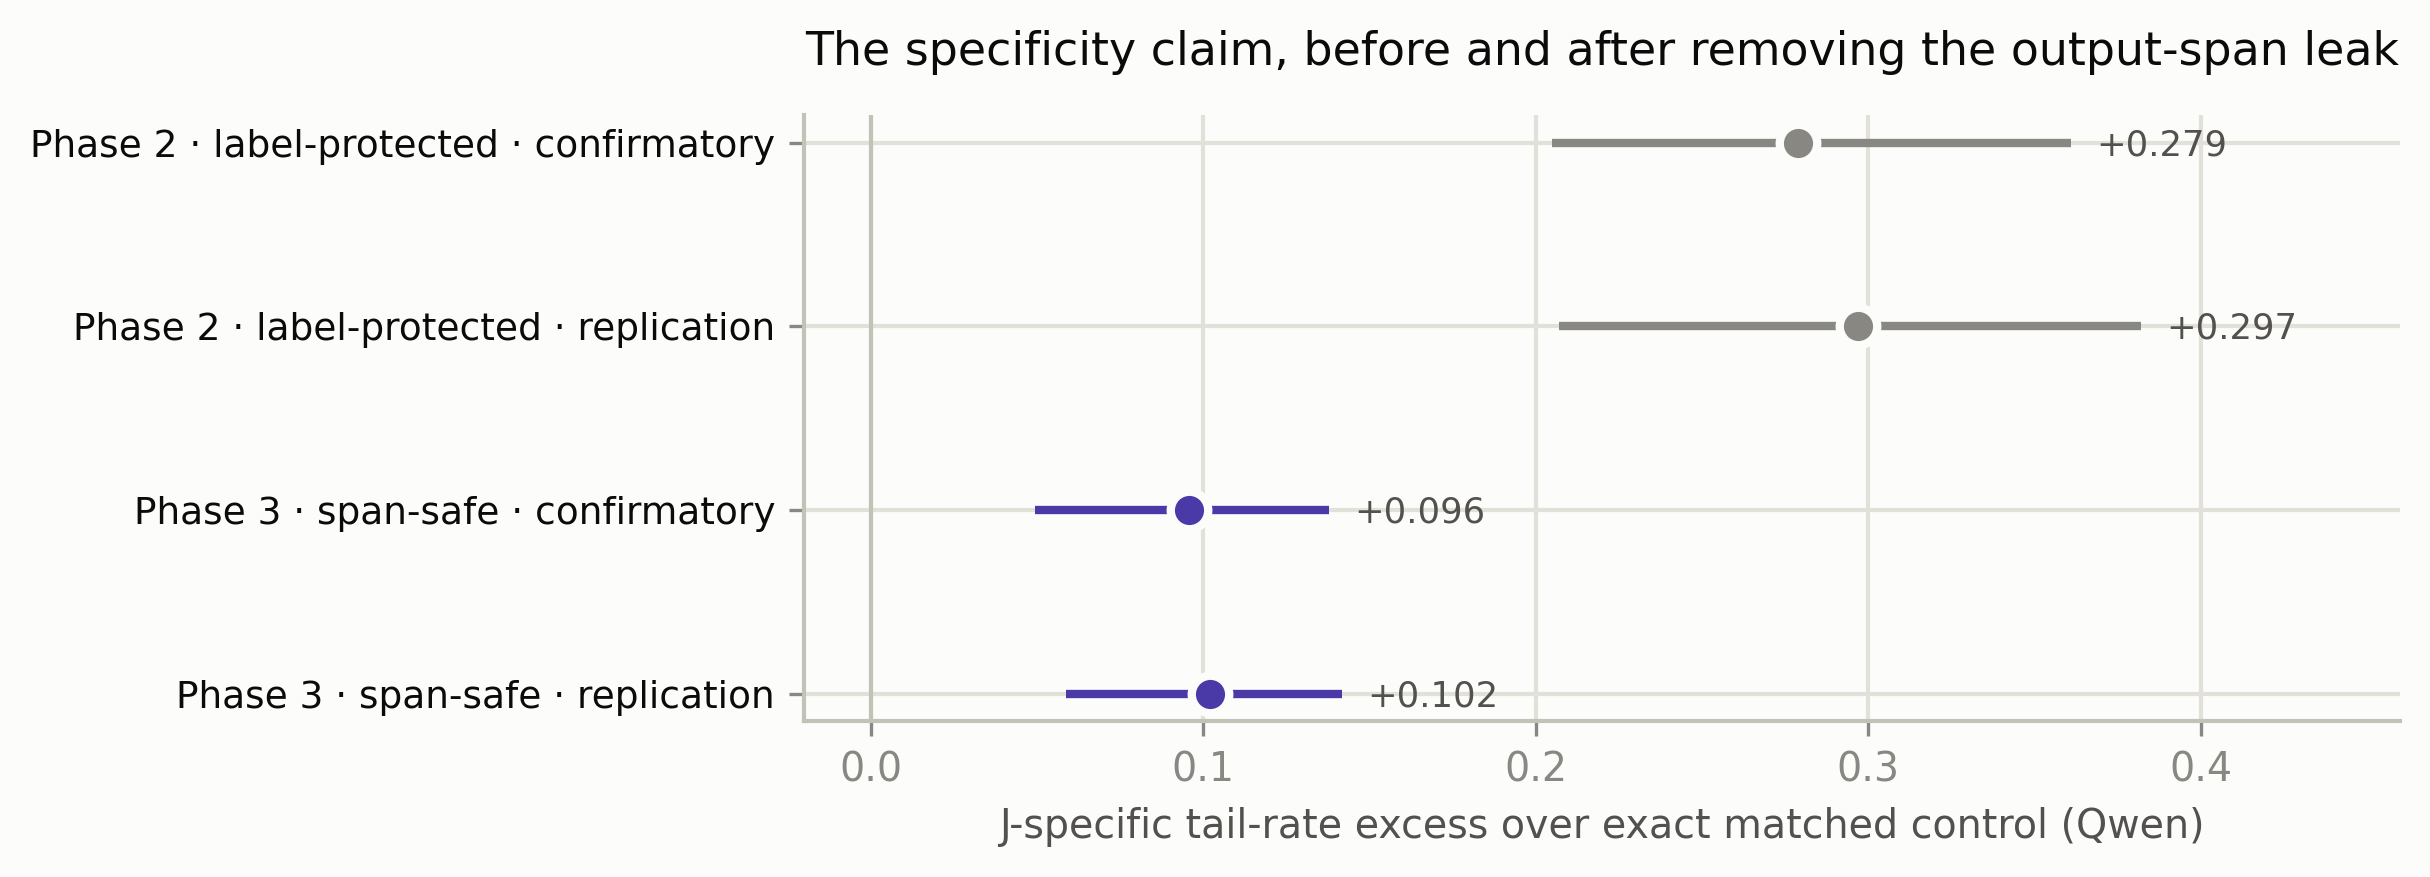
\includegraphics[width=\linewidth]{figures/figE_eras.png}
  \caption{The specificity estimand across eras: label-protected
  (Phase~2) vs span-safe (Phase~3), confirmatory and replication sides.
  The effect shrinks $\sim$$3\times$ when the output-span leak is
  removed --- and survives with $p\approx10^{-5}$.  Phase 3 CIs are
  family-clustered bootstrap (this paper's re-analysis).}
  \label{fig:eras}
\end{figure}

%----------------------------------------------------------------------------------------
\section{Controlled Composition}\label{sec:composition}

\todo{P3-P1 on the thick paired bank: contrast $-0.261$ nats,
wild-cluster CI $[-0.52, -0.01]$, $p=0.062$ at 17 intersection
families --- directional under the disclosed MDE, an honest near-miss
carried by the estimation targets \eid{p3-locked-analysis-v1}.
Replication side $-0.197$, $p=0.218$, same sign.  Think-vs-Instruct
on the thick bank indistinguishable ($+0.01$ $[-0.45,+0.39]$).
The workspace-word test: Qwen's contrast does NOT appear on the
in-context bank S ($+0.02$ $[-0.33,+0.42]$) --- per the pre-stated
decision rule the supportable noun is ``knowledge-access channel.''}

%----------------------------------------------------------------------------------------
\section{Mechanism: Bridge Mediation}\label{sec:mechanism}

The preregistered mediation primary (P3-P3, model chosen
magnitude-blind) rejects on Qwen: protecting the true bridge's token
directions rescues composed-item damage by $+0.431$ nats over
protecting a matched counterfactual bridge ($94$ composed items,
$p_{\mathrm{holm}}=0.018$) \eid{p3-locked-analysis-v1}
\tier{phase3-confirmatory}.  The seven-arm factorial
(Fig.~\ref{fig:mediation}) gives the mechanism-level picture:

\begin{itemize}
  \item \textbf{Qwen consumes its bridge channel.}  Deleting only the
  bridge's directions --- output fully preserved --- damages composed
  answers ($-0.89$, CI-clean); substituting the \emph{counterfactual}
  bridge's direction at matched energy is catastrophically worse than
  deletion ($-4.05$): the model reads what sits in the channel and
  follows it.  The unrelated-content lesion is nil ($-0.04$)
  \eid{p3-bridge-mediation-qwen36-27b-v1} \tier{phase3-development}.
  \item \textbf{Think does not.}  The swap is inert ($-0.09$), the
  rescue contrast mildly negative ($-0.20$ $[-0.38,-0.04]$)
  \eid{p3-bridge-mediation-olmo31-think-v1}.
\end{itemize}

\begin{figure*}[tbp]
  \centering
  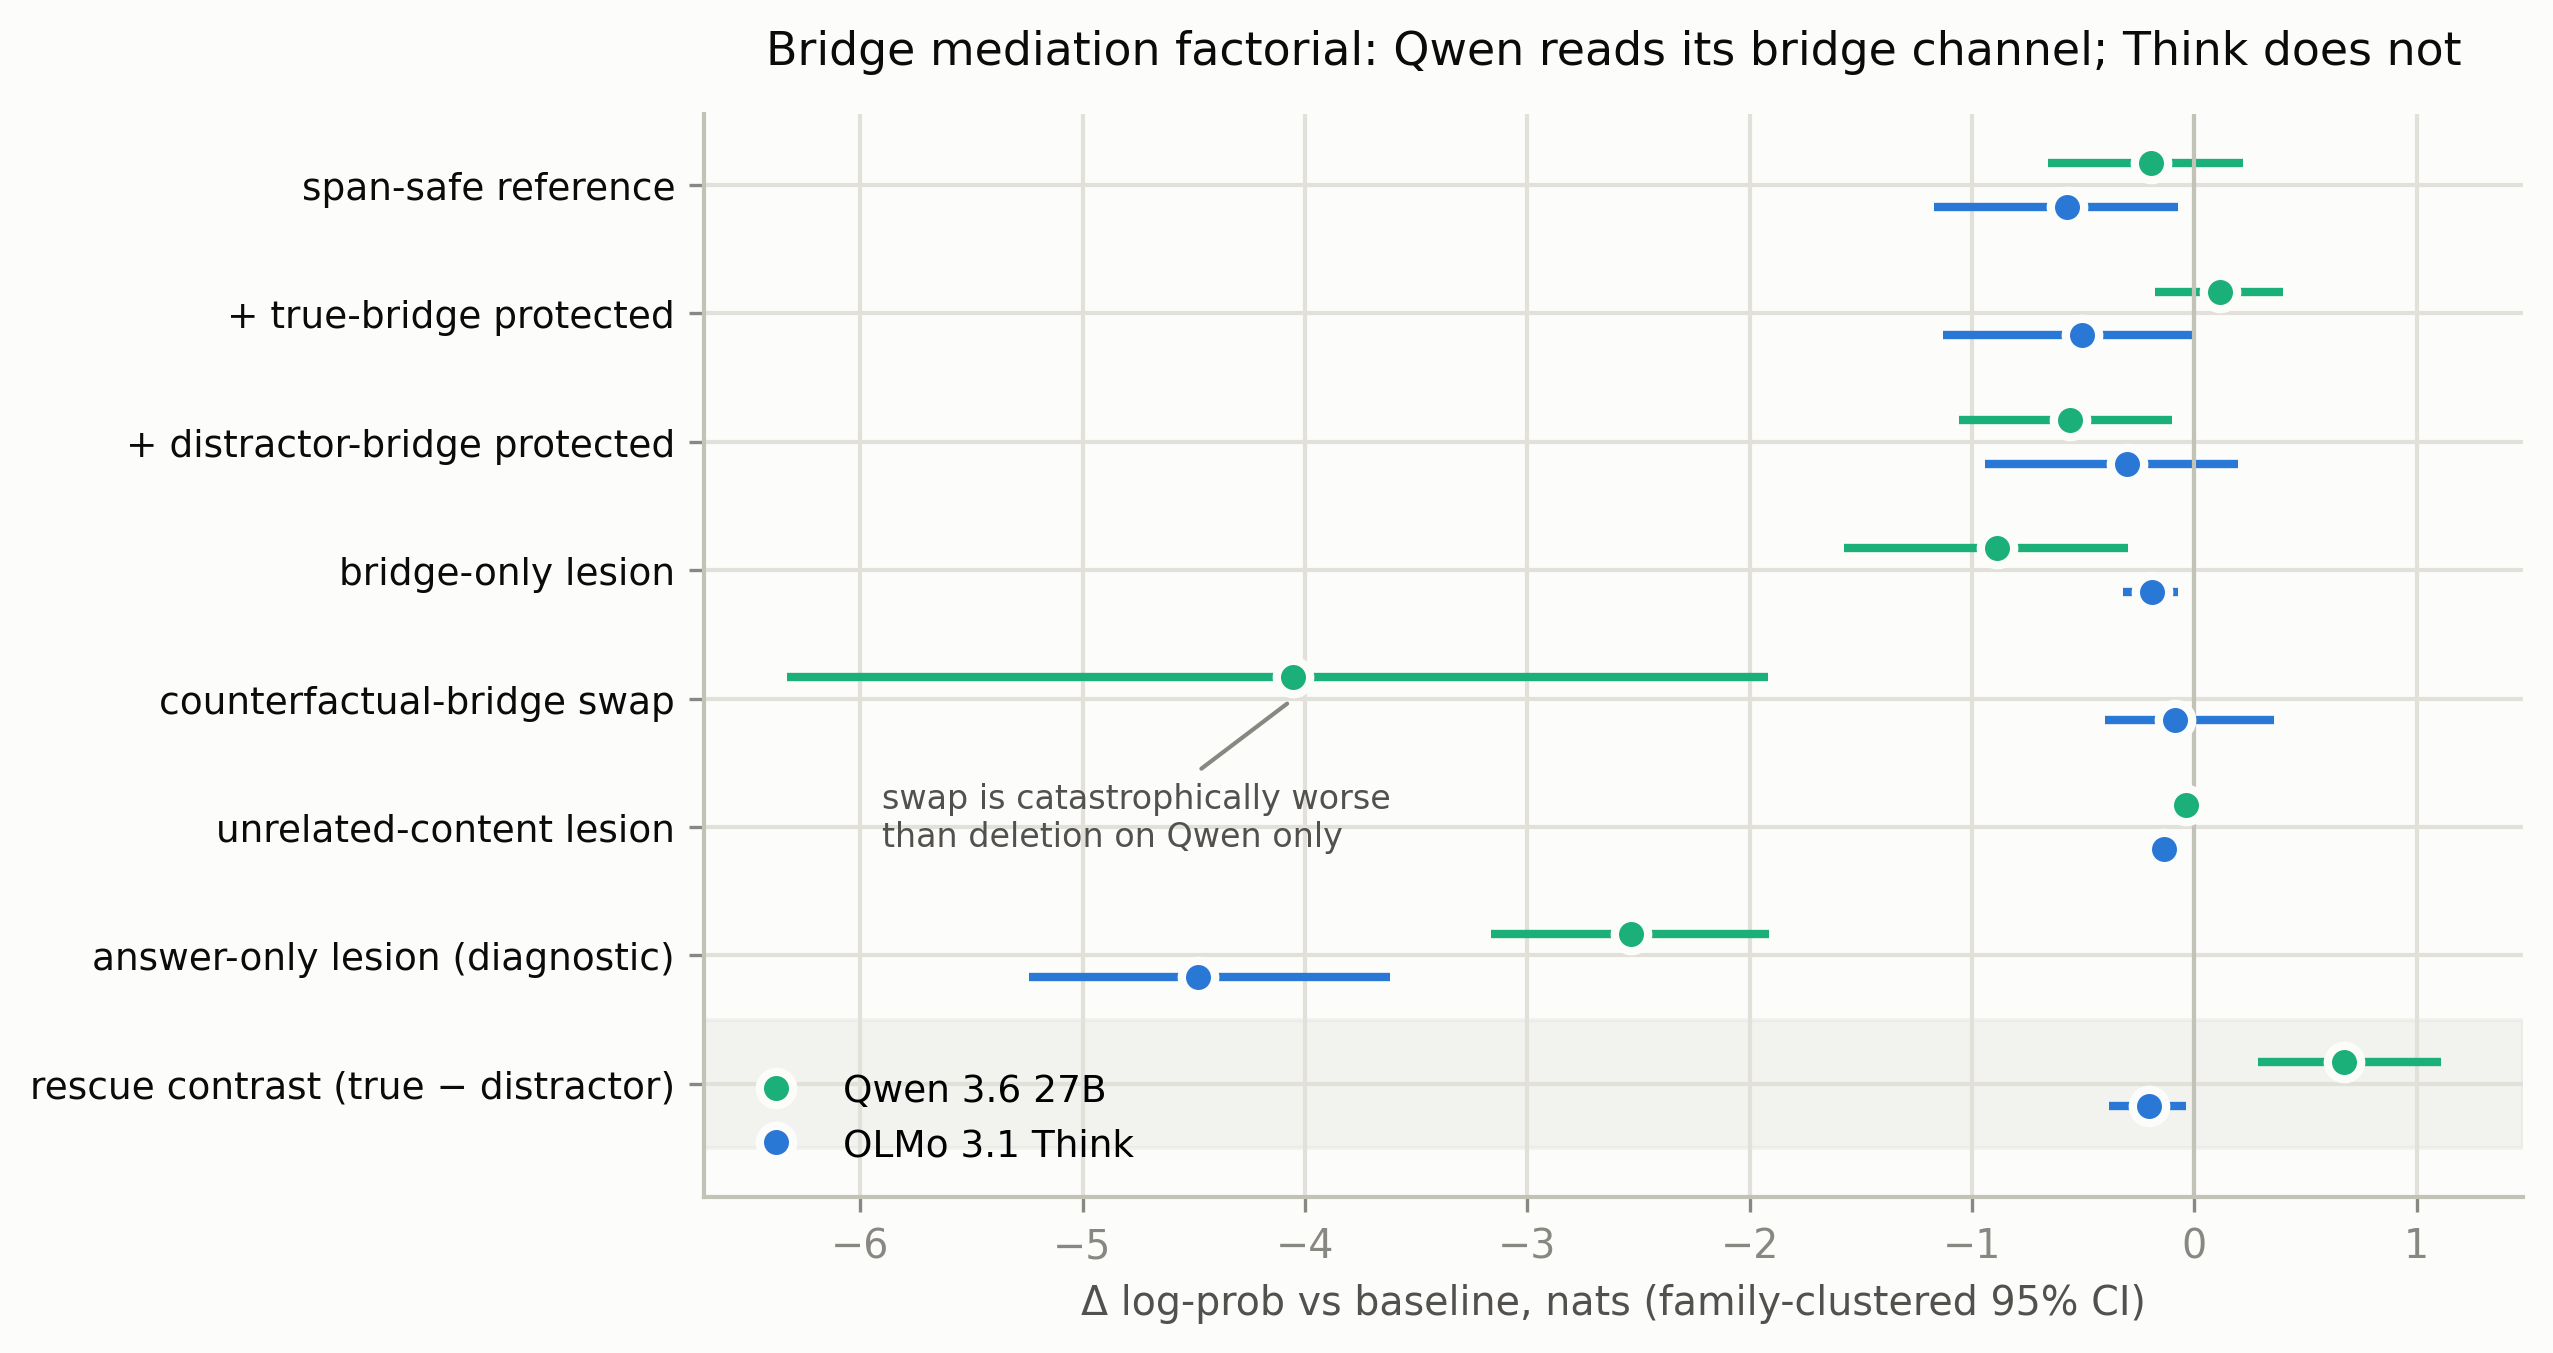
\includegraphics[width=0.92\linewidth]{figures/figC_mediation_forest.png}
  \caption{The bridge-mediation factorial (family-clustered 95\% CIs;
  40 Qwen / 20 Think composed items, span-safe base protection).  The
  same intervention grammar that shows Qwen routing composed answers
  through readable bridge content shows Think not doing so
  \eid{p3-bridge-mediation-*-v1} \tier{phase3-development}.}
  \label{fig:mediation}
\end{figure*}

\subsection{The accessibility organization}

\todo{The other half of the two-cluster picture: OLMo damage is
organized by output accessibility ($\rho=-0.30$/$-0.31$, CI-clean),
Qwen's by composition with the opposite sign ($+0.24$)
\eid{p3-overlap-mining-v1} \tier{phase3-development}.  Selection
pressure is a $12\times$ model property (blocked rows/position: Think
$1.33$, Instruct $1.22$, Qwen $0.10$) yet uncorrelated with damage
within model --- pressure and span geometry are dissociable.
Fig.~\ref{fig:access}.}

\begin{figure*}[tbp]
  \centering
  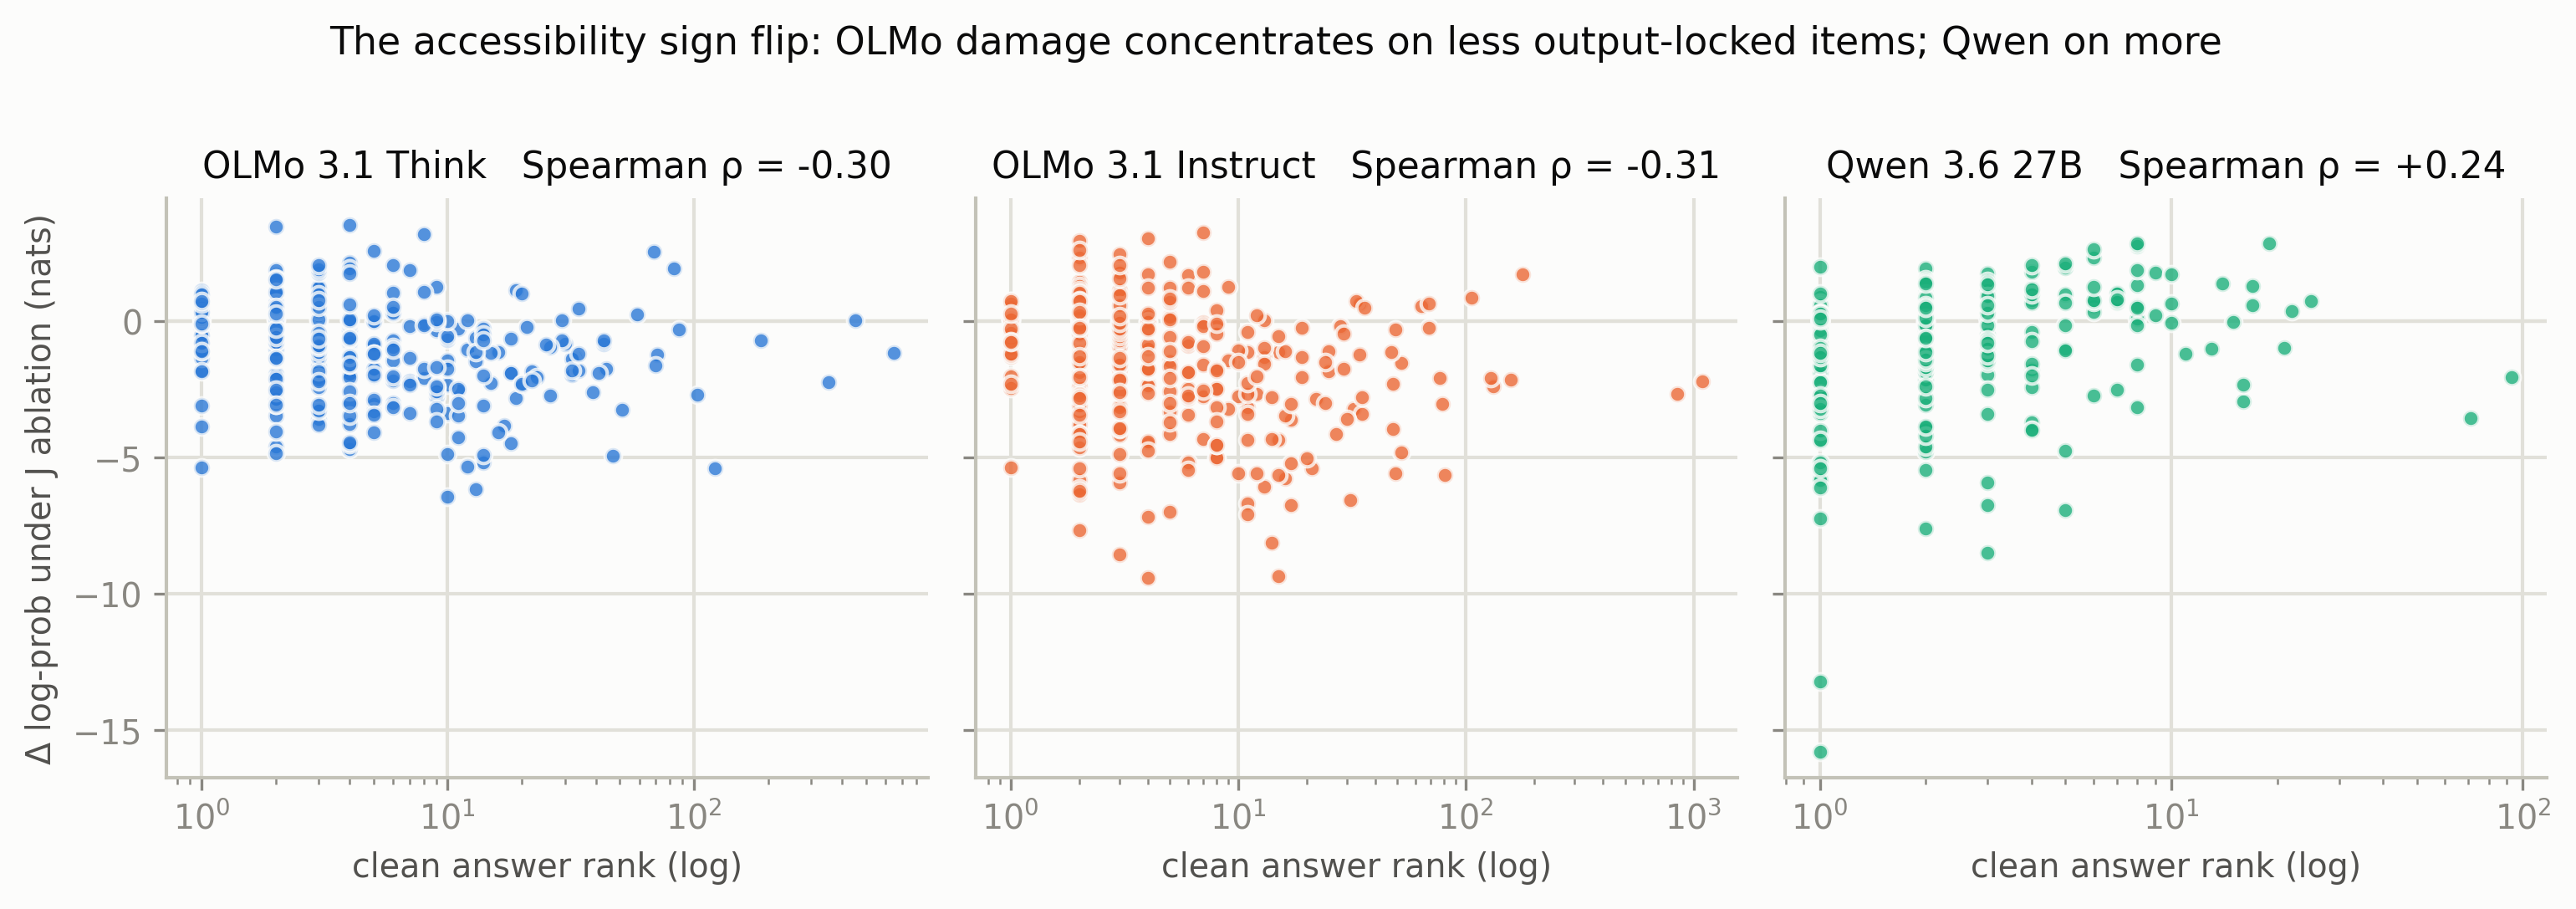
\includegraphics[width=\linewidth]{figures/figD_accessibility.png}
  \caption{Accessibility organization of J-ablation damage (975 frozen
  Phase 2 items).  On the OLMo pair, items whose answers are
  \emph{less} output-locked lose more; on Qwen the sign flips
  \eid{p3-overlap-mining-v1} \tier{phase3-development}.}
  \label{fig:access}
\end{figure*}

%----------------------------------------------------------------------------------------
\section{Prose Costs and Selectivity}\label{sec:prose}

\todo{Workstream C: the exact matched control Phase 2 never ran on
prose.  Prose cost is J-content everywhere, never dose (exact control
$+0.002$--$+0.021$/token vs label arm $+0.175$--$+0.945$); the
prose-cost ordering inverts the task ordering and tracks projector
overlap; span-safe removes $72$--$78\%$ of the label cost.  No model
earns ``selective'' wording at this tier
\eid{p3-prose-grid-figure-v1} \tier{phase3-development}.}

%----------------------------------------------------------------------------------------
\section{Reproducibility}\label{sec:repro}

\todo{The N8 ladder as a release gate: Level 1 narrative-blind
analysis reproduction ($\le5\times10^{-4}$ on all four primaries)
\eid{p3-n8-level1-repro-v1}; Level 2 sentinel cells bit-exact on all
three models \eid{p3-n8-level2-*-v1}; Level 3 one full 188-item Qwen
GPU cell bit-exact \eid{p3-n8-level3-qwen36-27b-v1} \tier{methods}.
Also: single-command repro, append-only evidence registry, frozen
partitions, preregistration with disclosed deviations.}

%----------------------------------------------------------------------------------------
\section{Discussion}\label{sec:discussion}

\todo{What is established: a readable, causally load-bearing,
content-specific J-channel on Qwen (knowledge-access channel), with
bridge mediation; an accessibility-organized content-channel response
on the OLMo pair; the instrument lesson (label vs span protection) as
a portable contribution for anyone using protected dynamic ablation.
What is not: the working-memory reading of ``workspace'' (fails the
bank-S test on both clusters); capacity-causes-shape (three assay-valid
models); any claim about consciousness.  Limitations: MDE on P3-P1;
development-tier arms of the factorial; two model families.}

\todo{Related work section (or fold into \S\ref{sec:problem}).}

%----------------------------------------------------------------------------------------

\begin{thebibliography}{9}

\bibitem[Anthropic, 2026]{Anthropic:Workspace}
Anthropic Interpretability Team.
\\\newblock \textit{Verbalizable Representations Form a Global
  Workspace in Language Models.}
\\\newblock transformer-circuits.pub/2026/workspace, July 2026.

\bibitem[Anthropic, 2026]{Anthropic:JLens}
Anthropic Interpretability Team.
\\\newblock \textit{jacobian-lens} (reference implementation).
\\\newblock github.com/anthropics/jacobian-lens, 2026.

\bibitem[OLMo Team, 2026]{AI2:OLMo3}
OLMo Team, Allen Institute for AI.
\\\newblock \textit{OLMo 3.1: Open Language Models.}
\\\newblock \todo{cite the actual OLMo 3.1 report}

\bibitem[Qwen Team, 2026]{Qwen:36}
Qwen Team.
\\\newblock \textit{Qwen 3.6 Technical Report.}
\\\newblock \todo{cite the actual Qwen 3.6 report}

\end{thebibliography}

\section*{AI Disclosure}
\todo{Adapt the standard disclosure: AI assistants used for run
orchestration, analysis tooling, formatting, and proofreading; all
design decisions, experimental results, and final content are my own.}

\section*{Code and Data Availability}
Analysis code, the evidence registry, and small metrics are in the
\texttt{labs} repository under \texttt{interpretability/} (packages
\texttt{jspace\_part2}, \texttt{jspace\_phase3}); heavy artifacts
(fitted lenses, per-item parquets, generation traces) are archived in
the run store.  Every primary quantity regenerates via the packages'
single-command reproduction entry points.

\end{document}
